%############################################################################
\chapter{\AutoProof: a Tool for Auto-active Verification}
\label{sec:ap}
\chapterimage{images/autoproof}
%############################################################################


This chapter describes \AutoProof, our auto-active verifier for functional properties of object-oriented programs.
In its latest development state, \AutoProof offers a unique combination of features that make it a powerful tool in its category and a significant contribution to the state of the art.
\AutoProof targets a real complex object-oriented programming language (Eiffel)---as opposed to more abstract languages designed specifically for verification.
It supports most language constructs, as well as a full-fledged verification methodology for heap-manipulating programs based on a flexible annotation protocol, sufficient to completely verify a variety of programs and verification challenges that are representative of object-oriented idioms as used in practice (see Chapter~\ref{sec:method}).
\AutoProof was developed with usability and extensibility in mind: it features techniques to help debug failed verification attempts so as to offer an incremental user experience, its annotation library can be augmented with new abstract models, and its implementation can be easily adapted to accommodate changes in the input language.


%############################################################################
\section{Introduction}
\label{sec:ap-intro}
%############################################################################


\AutoProof is an auto-active verifier of functional correctness working on Eiffel programs and using Boogie~\cite{LEINO08} as a back-end verifier. Figure~\ref{fig:ap-workflow} shows the general workflow of using \AutoProof. It takes compiled Eiffel programs annotated with contracts and translates them to Boogie code. The Boogie verifier is then invoked on the generated Boogie code transforming the intermediate Boogie program to verification conditions. These verification conditions are finally checked by an SMT solver (currently Z3). The result of the verification is then traced back to Eiffel code and displayed to the user.

\begin{figure}[!htb]
\centering
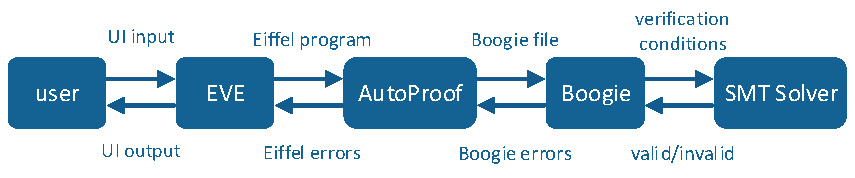
\includegraphics[width=\columnwidth,page=1]{images/drawings.pdf}
\caption{High-level overview of the \AutoProof verification workflow.}
\label{fig:ap-workflow}
\end{figure}

\AutoProof does modular verification on the level of routines. Each routine is checked separately and for calls inside a routine only the callee's specification is used. This allows to verify Eiffel systems piece by piece, and, when a routine body is changed, only the changed routine must be reverified. \AutoProof is available online as well as integrated in \EVE, the Eiffel Verification Environment IDE~\cite{EVE}.

